\section{Timeliness to Supersafety}

In this section we construct a supersafe protocol
$\Pi^*$ using a black-box reduction from a safe, live($u$) and timely($v$)
protocol $\Pi$.
Each honest party $P^*$, executing the $\Pi^*$ protocol, runs a
full node party $P$ of protocol $\Pi$.
The ledger of party $P$ and $P^*$, at round $r$, are denoted as $\Ledger[][][r]$ and
$\Ledger[*][][r]$ respectively.
The main idea is that $P^*$ constructs ledger $\Ledger[*][][r]$
by filtering through ledger $\Ledger[][][r]$, and only keeps transactions
with recorded round less than or equal to $r - v$. When a transaction
is written to $P^*$, it is simply forwarded to $P$. This process is illustrated
in Figure~\ref{fig:reduction-timeliness-supersafety}.

\begin{figure}
  \centering
  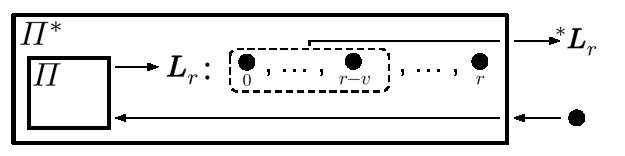
\includegraphics[width=0.9\columnwidth,keepaspectratio]{figures/reduction-timeliness-supersafety.pdf}
  \caption{The reduction from Timeliness
    (the $\Pi$ protocol) to Supersafety (the $\Pi^*$ protocol). A transaction is illustrated
    as a black circle and its recorded round is displayed below.
  }

 \label{fig:reduction-timeliness-supersafety}
\end{figure}

\atnote{Add \now notation}
\atnote{Add set builder notation for sequences}
The pseudocode of protocol $\Pi^*$ is illustrated in Algorithm~\ref{alg:reduction-timeliness-supersafety}.
When the \rread function is invoked, the temporal ledger of party $P$ is acquired
in Line~\ref{line.reduction-t-s-ledger}.
Then, transactions with recorded round less than or equal to $\now - v$ are
filtered to create $\Ledger[*]$, which is returned in Line~\ref{line.reduction-t-s-filter}.
When the \wwrite function is invoked with transactions $\tx$, party $P^*$ simply writes $\tx$
to party $P$ in Line~\ref{line.reduction-t-s-write}.

\import{./}{algorithms/algorithm-reduction-timeliness-supersafety.tex}

\begin{lemma}[Past Perfect]\label{lem:past-perfect}
  Consider a temporal ledger protocol $\Pi$'s
  execution with duration $R$ rounds in which $\Pi$ is
  safe, live($u$), and timely($v$).
  If for some honest party $P_1$ and some round $r_1$ it holds that
  $(r^*, \tx) \in \Ledger[P_1][][r_1]$, then
  for all honest parties $P_2$ and for all rounds $r_2 \geq r^* + v$
  it holds that $(r^*, \tx) \in \Ledger[P_2][][r_2]$,
  as long as at least one new honest transaction $\tx'$ appears in the
  network at any round $r_3$, where $r_1 < r_3 \leq R - u$.
\end{lemma}
\begin{proof}
  Consider an execution as in the statement and suppose, towards a contradiction,
  that $(r^*, \tx) = \Ledger[P_1][][r_1][k]$ for some $k \in \mathbb{N}$,
  but $(r^*, \tx) \not\in \Ledger[P_2][][r_2]$
  with $r_2 \geq r^* + v$.
  From safety,
  $\Ledger[P_2][][r_2] \prec \Ledger[P_1][][r_1]$ and
  $|\Ledger[P_2][][r_2]| \leq k < |\Ledger[P_1][][r_1]|$.
  Due to liveness, $(r', \tx') = \Ledger[P_2][][r_3 + u][k']$,
  for some $r', k' \in \mathbb{N}$.
  As $\tx'$ is new, it is not in $\Ledger[P_1][][r_1]$.
  Due to safety, $k' \geq |\Ledger[P_1][][r_1]| > k$, and
  $\Ledger[P_2][][r_3 + u][k] = (r^*, \tx)$.
  Therefore
  $(r^*, \tx) \in \Ledger[P_2][][r_3 + u][|\Ledger[P_2][][r_2]|{:}]$.
  Since $r^* \leq r_2 - v$, this contradicts the timeliness with parameter $v$.\Qed
\end{proof}

\atnote{Adjust for $R - u$?}
\begin{conjecture}
  An execution of protocol $\Pi^*$ is supersafe, if the execution of the
  temporal ledger protocol $\Pi$ is safe, live($u$) and timely$(v)$.
\end{conjecture}
\begin{proof}
  Consider any honest parties $P_1^*,P_2^*$ and any round $r$.
  Let $(r^*, \tx) \in \Ledger[P_1][][r]$, where $r^* \leq r - v$.
  From Lemma~\ref{lem:past-perfect} it holds that
  $(r^*, \tx) \in \Ledger[P_2][][r]$.

\end{proof}

\dznote{Figure}
\dznote{Describe and prove the forward reduction}
\dznote{Describe and prove the reverse reduction}
